\documentclass[11pt,unknownkeysallowed,usenames,dvipsnames]{beamer}
\usepackage[utf8]{inputenc}
\usetheme{metropolis}

% A font that I found more "classy" than the default one ...
% -- just comment the three next lines if you hate it ;)
\usepackage{libertine}
\renewcommand*\familydefault{\sfdefault}
\usepackage[T1]{fontenc}

% Packages
\usepackage{amsmath}
\usepackage{hyperref}
\hypersetup{colorlinks,breaklinks,
    urlcolor=teal,linkcolor=teal,citecolor=teal}
\graphicspath{{img/}}

% Beamer settings
\setbeamercolor{block title}{bg=gray!30}
\setbeamercolor{block body}{bg=gray!10}
\setbeamersize{text margin left=16pt,text margin right=16pt}

% Set minted options
%\usepackage{minted}
%\newminted{python}{fontsize=\scriptsize, 
%    linenos=false,
%    numbersep=8pt,
%    gobble=4,
%    bgcolor=gray!10,
%    fontfamily=courier}

% Title and ...
\title{An introduction to Python}
\author{Thibaut Lunet, Aitor Pérez}

\date{March 19, 2018}

\begin{document}
	\maketitle
    
	\begin{frame}{What are we talking about}
        \begin{block}{A little history}
            \begin{itemize}
            \item Programming language conceived by a Monty Python fan in the 80's
            \item First released in 1991, then
            \begin{itemize}
                \item Python 2 in 2000 (community backed development, support $\rightarrow$ 2020)
                \item Python 3 in 2008 (major revision)
            \end{itemize}
            \end{itemize}
            Current versions (2.7, 3.6) are not entirely compatible, 
            but very close
        \end{block}
        
        \begin{block}{Main motivations}
            Developers wanted to create a language that would be
            
            \vspace{-10pt}
            \begin{itemize}
                \item general purpose (they really got that !)
                \item highly extensible and modular (dynamic language)
                \item beautiful, simple, \textbf{easily readable}
               \end{itemize} 
        \end{block}
        
        \vspace*{-20pt}
	\end{frame}
    
	\begin{frame}{Functioning principles}
        \begin{block}{Pre-compilation of code files}
            \centering
            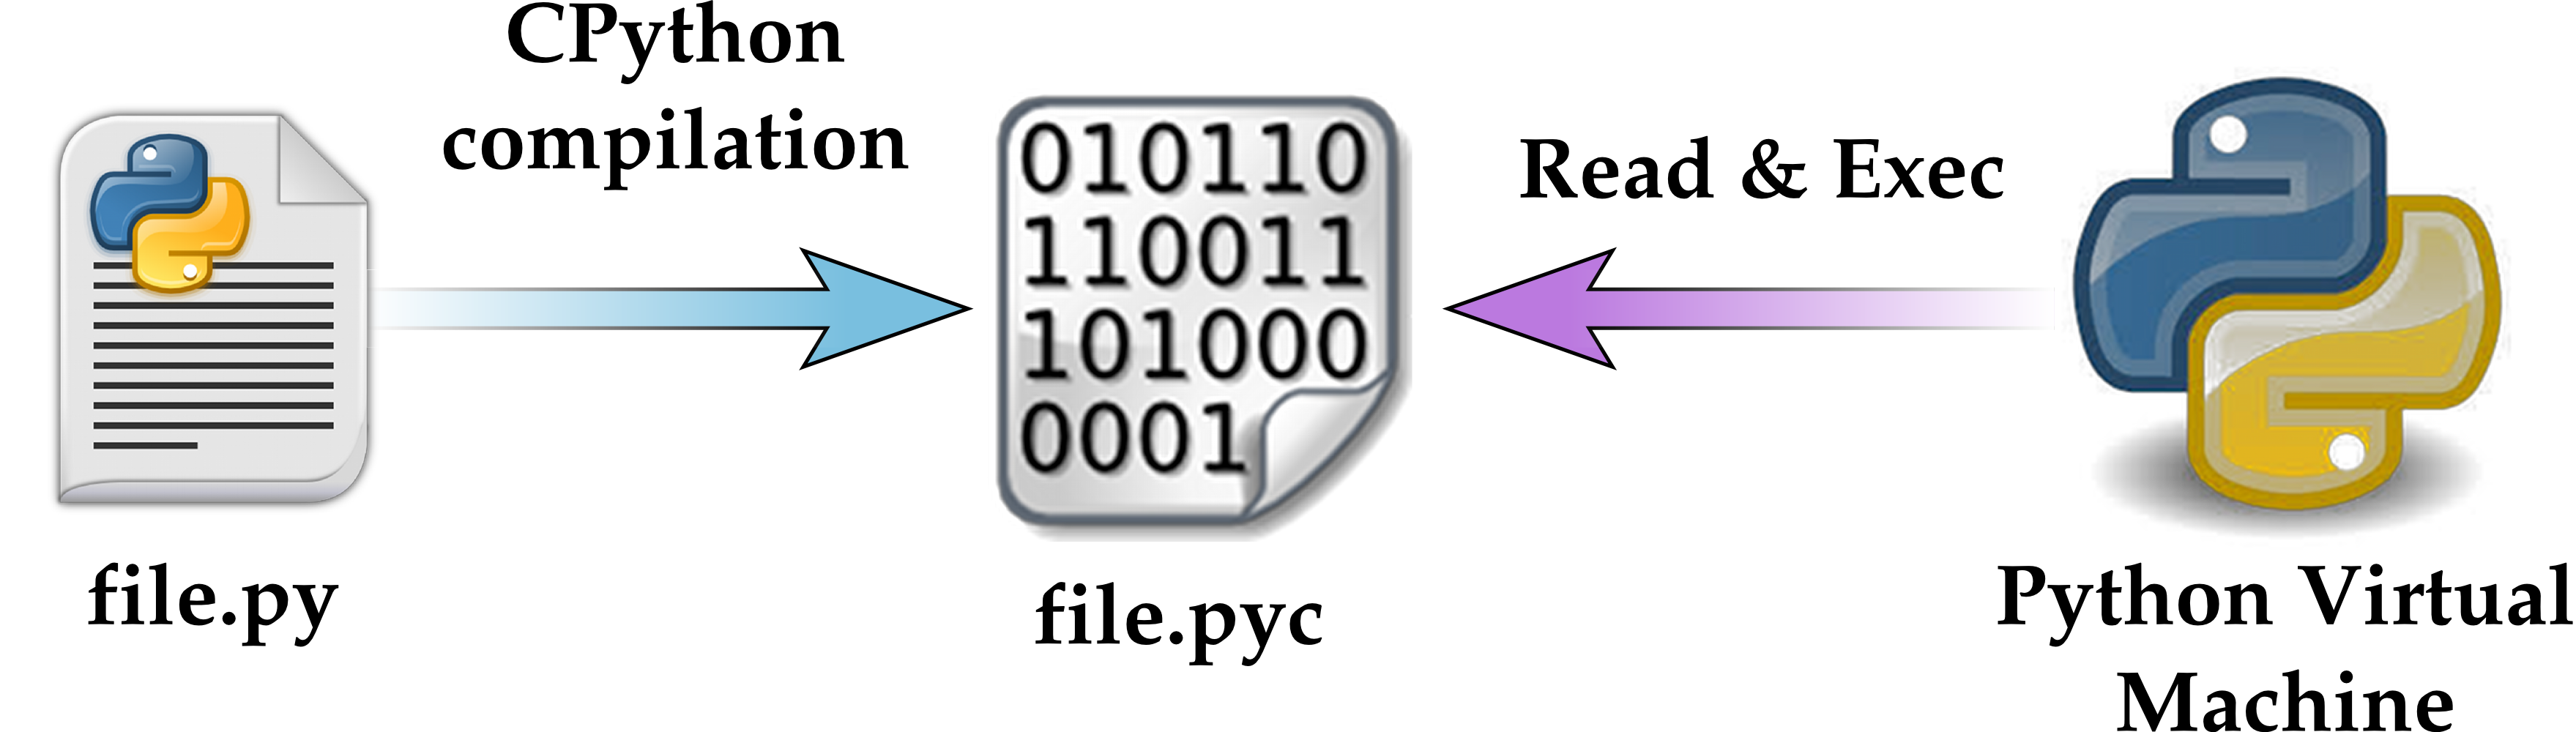
\includegraphics[width=0.8\linewidth]{cpython}
            
            \vspace*{-20pt}   
            \begin{itemize}
                \item Allows partial code optimization
                \item Totally transparent to user
                \item Portability on every architecture
            \end{itemize}
        \end{block}
        Python core (Virtual Machine) is written in C:
        
        \vspace*{-5pt}
        \begin{itemize}
            \item Easy interface with other compiled languages (C/C++, Fortran)
            \item Same speed for read/write files as C
        \end{itemize}
        
        \vspace*{-20pt}
    \end{frame}

	\begin{frame}{Python vs. Others (Matlab, Fortran, C/C++, ...)}
        \begin{itemize}
            \item License-free and open-source ($\neq$ Matlab)
            \item Huge users community, many (free) packages for many applications
            \item Extremely easy of use for non-I-love-programming people \\ ($\neq$ Fortran, C/C++)
            \item Computation can be accelerated using Fortran or C/C++
            library ... 
            \item Can scale to very large problems (parallel computing, ...)
            \item Structured and friendly ways for developing library ($\neq$ Matlab)
        \end{itemize}
%		Some drawbacks of MATLAB:
%		\begin{itemize}
%			\item It is a proprietary software
%			\item It does not scale properly to big projects
%			\item Hard to work with in a general framework other than numerical computing
%			\item Tricky code organization (function name = file name)
%			\item Toolboxes are distributed/purchased separately
%		\end{itemize}
	
		\vspace{10pt}
	
		\begin{center}
            Python = many advantages, with very few drawbacks !
        \end{center}
	\end{frame}

	\begin{frame}{Practical tools}
        \vspace{5pt}
        \begin{block}{Using python console}
        \centering
        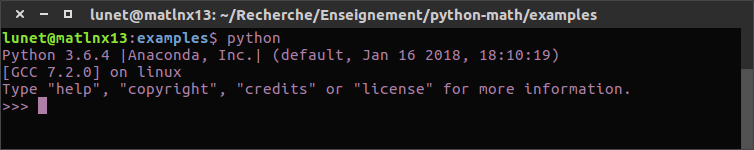
\includegraphics[width=0.95\linewidth]{python-terminal}
        \end{block}
        
        \begin{block}{Running a script}
        \centering
        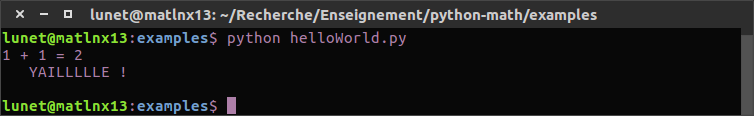
\includegraphics[width=0.95\linewidth]{python-script}
        \end{block}
        \vspace{-10pt}
        \begin{center}
            All-in-One solution $\Rightarrow$ \textbf{Spyder} !
        \end{center}
        \vspace{-10pt}
	\end{frame}
    
    
%\defverbatim[colored]\pythonCode{
%\begin{pythoncode}     
%       
%    # Integer
%    i1 = 1
%    i2 = 7 % 3  # i2 = 1
%    
%    # Float -- by default, double precision !
%    f1 = 0.5 
%    f2 = f1/7  # f2 = 0.07142857142857142
%    
%    # Complex
%    c1 = 1+1j
%    c2 = c1 + f1 + i1  # Automatic conversion, c2 = 2.5 + 1j
%    
%    # String
%    s1 = 'salut'
%    s2 = 'toi'
%    s3 = s1 + s2  # s3 = 'saluttoi'
%    
%    # Boolean
%    b1 = True
%    b2 = (i1 != 1)*b1 + (i1 == 1)*(f1 < 10)*(f2 >= 0)  # b2 = True
%        
%\end{pythoncode}
%}    
\begin{frame}{Basic variables types and operations}
%    \pythonCode
    Slide codes at: 
    \href{https://gitlab.unige.ch/Thibaut.Lunet/python-math/tree/master/examples/code-examples}{python-math/examples/code-examples.py}
    
    \vspace*{5pt}
    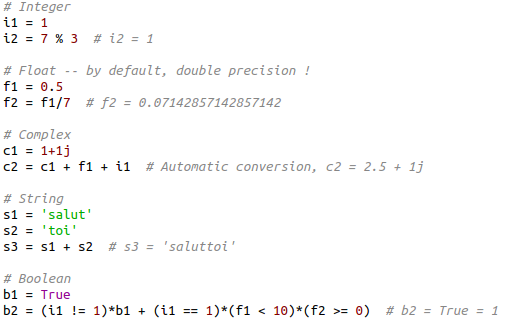
\includegraphics[width=0.9\linewidth]{code-basic-variables}
\end{frame}



%\defverbatim[colored]\pythonCode{
%\begin{pythoncode}           
%    # List
%    l1 = [1, 2, 5, 6]
%    # Access elements : l1[0] = 1, l1[2] = 5, l1[-1] = 6 
%    # Slice : l1[1:3] = [2, 5]
%    
%    # Nested list
%    l2 = [ ['vive', 'la'], ['saucisse', 2], 'Toulouse']
%    # Extract sub-list : l2[0] = ['vive', 'la'] 
%    # Access element : l2[0][1] = 'la', l2[1][0] = 'saucisse'
%    
%\end{pythoncode}
%}    
\begin{frame}{Lists}
%    \pythonCode\vspace{-20pt}
    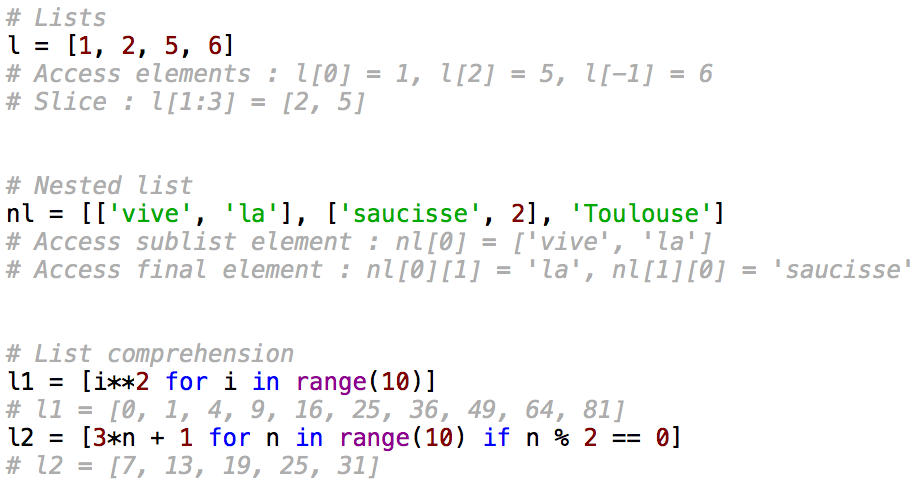
\includegraphics[width=0.9\linewidth]{code-lists}
\end{frame}


\begin{frame}{Dictionary}
    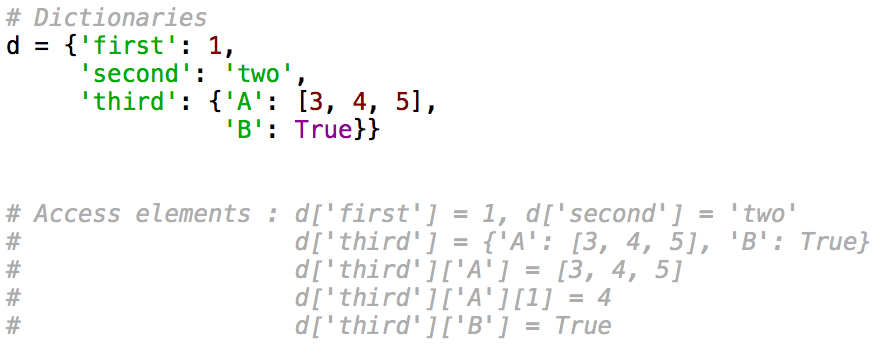
\includegraphics[width=0.9\linewidth]{code-dictionaries}
\end{frame}


%\defverbatim[colored]\pythonCode{
%\begin{pythoncode}           
%    # For loop
%    for i in range(5):
%        print('i = {}'.format(i))
%        
%    # If condition
%    if 1 == 2:
%        print('Tocard')
%    elif 1 == 0:  # Not mandatory
%        print('Toujours pas')
%    else:  # Not mandatory
%        print("OK d'accord")
%        
%    # While loop
%    i = 0
%    while i < 10:
%        print('TAIHOOO-'+str(i))
%        i += 1
%        if i == 5:
%            break  # Allows to escape from the while loop
%    
%\end{pythoncode}
%}    
\begin{frame}{Conditional structures}
    \vspace{-5pt}
    \begin{center}
        \textbf{Tabs matter !}
    \end{center}
    \vspace{-5pt}
%    \pythonCode
    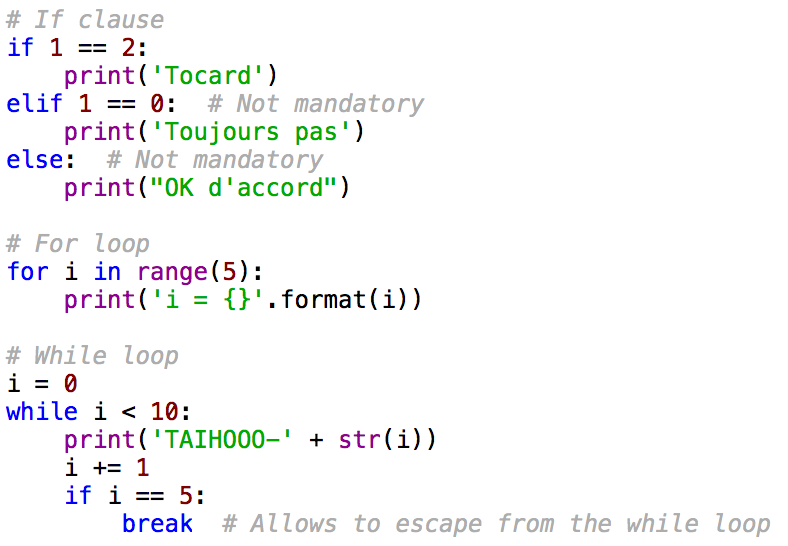
\includegraphics[width=0.8\linewidth]{code-conditional-structures}

\end{frame}



%\defverbatim[colored]\pythonCode{
%\begin{pythoncode}           
%    def funcA(a, b=1):
%        return a + b
%    # funcA(0.5, 2) = funcA(0.5, b=2) = 2.5
%    # funcA(1) = 1.5
%    # funcA() -> ERROR
%    
%\end{pythoncode}
%}
\begin{frame}{Function definition}
    %\pythonCode
    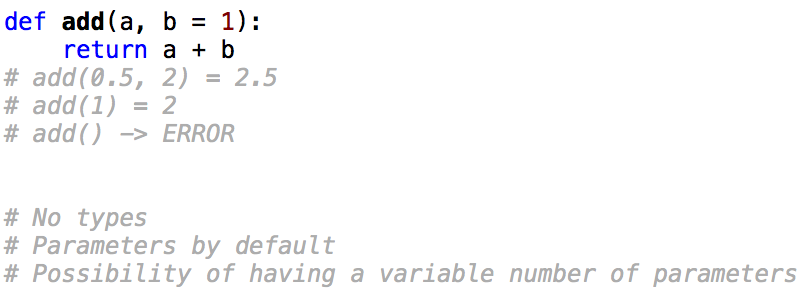
\includegraphics[width=\linewidth]{code-functions}
\end{frame}
   

\begin{frame}{File I/O}
	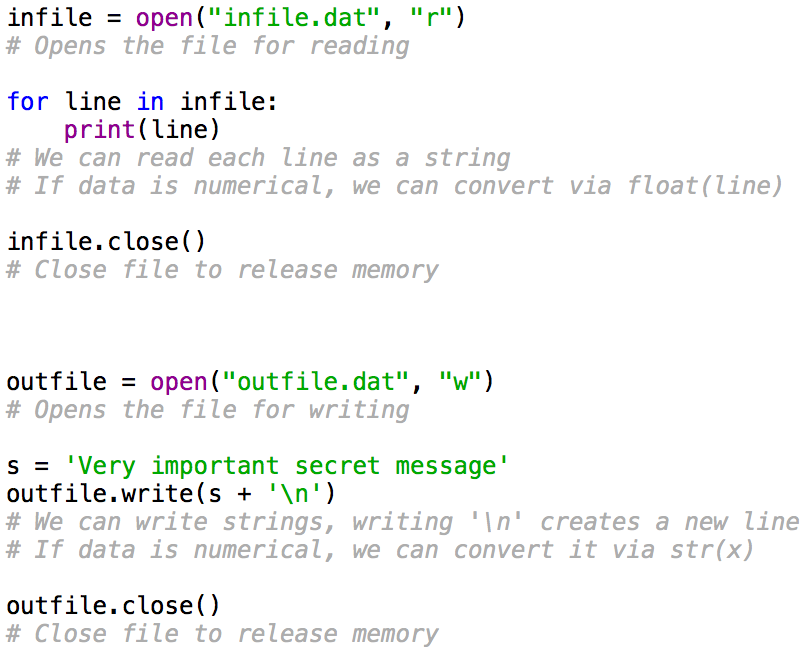
\includegraphics[width=0.8\linewidth]{code-fileio}
\end{frame}


\begin{frame}{Numpy and Scipy, what for ?}
	\begin{center}
        Loops in python are (REALLY) slow\\
        $\Rightarrow$ do algebraic computation in C (or Fortran)
    \end{center}
    \begin{block}{Numpy : interface for array manipulation}
        \begin{itemize}
            \item Data stored in contiguous memory location
            \item Operations on arrays in C
            \item Uses optimized C library for algebraic computation (BLAS)
        \end{itemize}
    \end{block}
    \begin{block}{Scipy : companion package for scientific computing}
        \begin{itemize}
            \item Many functions for linear algebra, optimization, interpolation, ...
            \item Interface with C and Fortran optimized routine\\
            (LAPACK, FFTW, QUADPACK, ... and many others !)
            \item See \href{https://docs.scipy.org/doc/scipy/reference/tutorial/}{Scipy tutorials} on the Internet
        \end{itemize}
    \end{block}
\end{frame}

\begin{frame}{Numpy basics I}
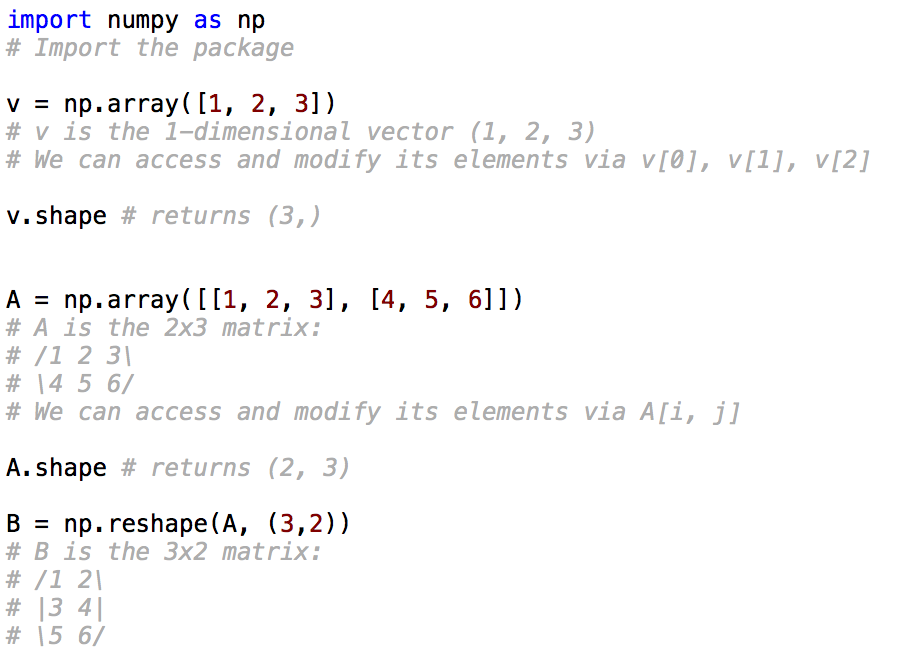
\includegraphics[width=0.9\linewidth]{code-numpy1}
\end{frame}

\begin{frame}{Numpy basics II}
	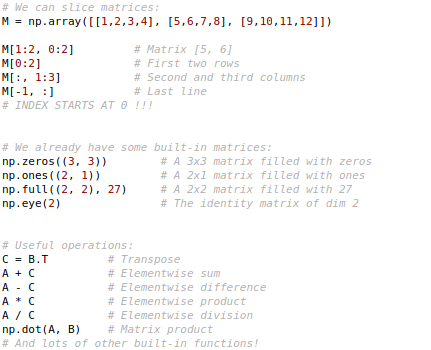
\includegraphics[width=0.8\linewidth]{code-numpy2}
\end{frame}

\begin{frame}{Data visualization with Matplotlib I}
    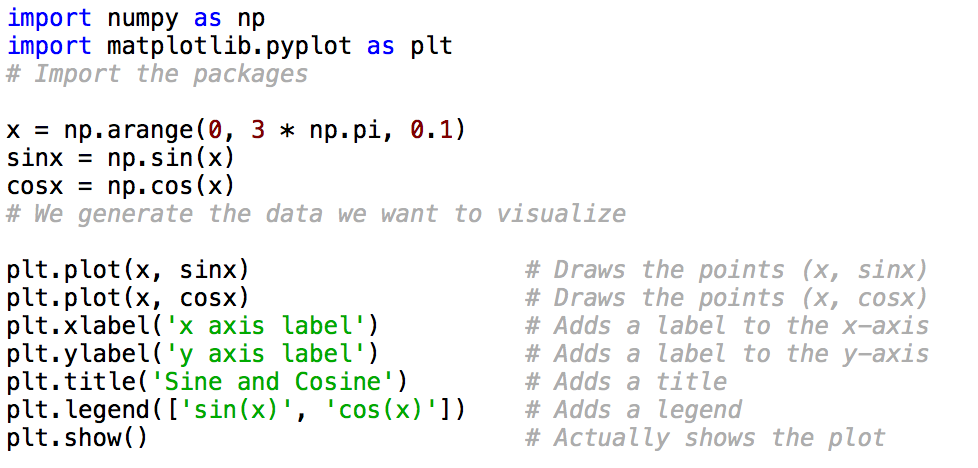
\includegraphics[width=0.8\linewidth]{code-matplotlib1}
    
	\centering    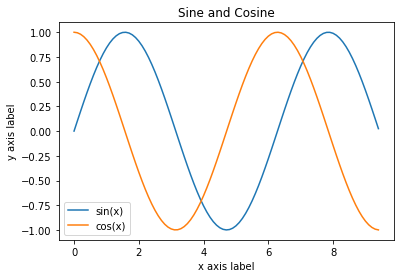
\includegraphics[width=0.4\linewidth]{plot1}
\end{frame}

\begin{frame}{Matplotlib II}
	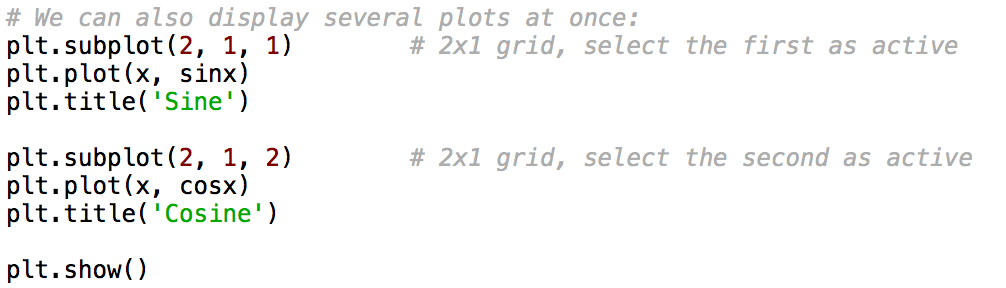
\includegraphics[width=0.9\linewidth]{code-matplotlib2}
	
	\centering    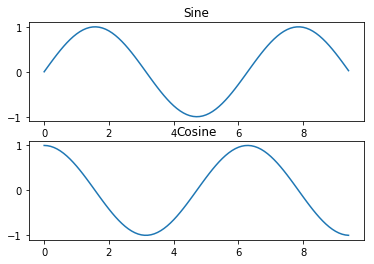
\includegraphics[width=0.4\linewidth]{plot2}
    
    ... and more in    
    \href{https://gitlab.unige.ch/Thibaut.Lunet/python-math/tree/master/examples/matplotlib}{python-math/examples/matplotlib} directory
\end{frame}

\begin{frame}{To go further with Numpy and Scipy}
	% 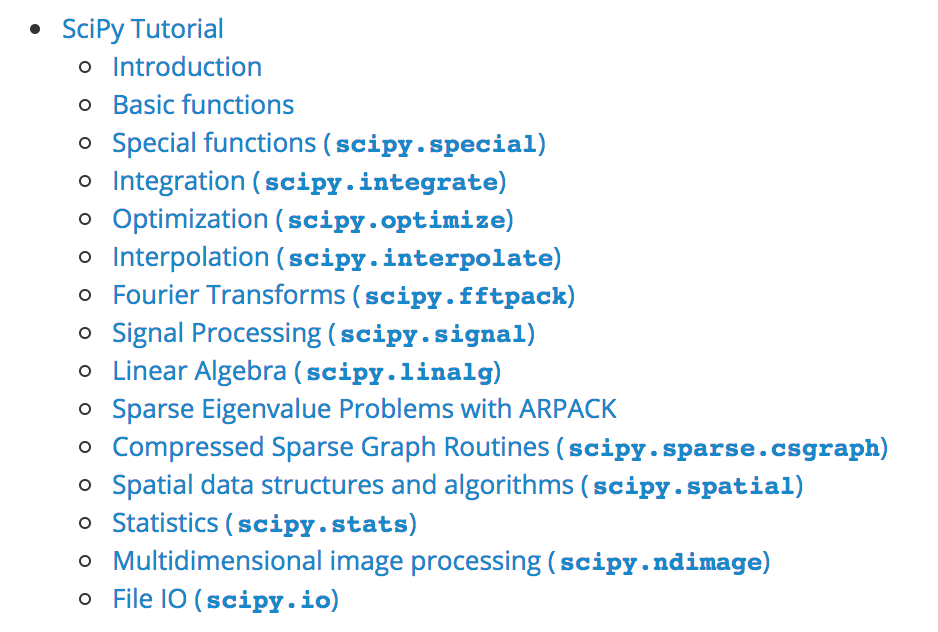
\includegraphics[width=0.9\linewidth]{code-scipy}
	\small
	\vspace{5pt}
	\begin{block}{Numpy examples :}
		\begin{itemize}
			\item Call Fortran routines to accelerate computations
			\item Easily read and write files with single line coding
		\end{itemize}
	\end{block}
	\vspace*{-7pt}
	... and more in    
	\href{https://gitlab.unige.ch/Thibaut.Lunet/python-math/tree/master/examples/numpy}{python-math/examples/numpy} directory
	\vspace*{6pt}
	\begin{block}{Scipy examples :}
		\begin{itemize}
			\item Data regression using least square minimization
			\item Eigenvalue computation of the tri-dimensional advection operator
		\end{itemize}
	\end{block}
	\vspace*{-7pt}
	... and more in    
	\href{https://gitlab.unige.ch/Thibaut.Lunet/python-math/tree/master/examples/scipy}{python-math/examples/scipy} directory \\
\end{frame}

\begin{frame}{Sympy, more than just another py-word game}
    If you are interested in
    \begin{itemize}
        \item Sparing few neurons by not doing computation by hand
        \item Verifying some solutions you will give to students
        \item Obtaining a direct latex translation of some ugly formula 
    \end{itemize}
    \begin{center}
        Sympy can help you !
    \end{center}
    \begin{itemize}
        \item Symbolic optimized computation core in python
        \item Can combine numerical calculation with Numpy
        \item Allow some nice output form within Spyder
    \end{itemize}
\end{frame}

\begin{frame}{To go further with Sympy}
	\begin{block}{Scipy examples :}
        \begin{itemize}
            \item Block matrix computation with non-commutative elements
            \item Compute interpolation formula for non-structured grid
            \item Latex translation of symbolic formula
        \end{itemize}
    \end{block}
    \vspace*{-7pt}
    ... and more in    
    \href{https://gitlab.unige.ch/Thibaut.Lunet/python-math/tree/master/examples/sympy}{python-math/examples/sympy} directory \\
    See also \href{http://docs.sympy.org/latest/tutorial/index.html}{Sympy Tutorials} on the Internet
\end{frame}

\begin{frame}{Conclusion}
    Here was just presented a tiny part of python application for researchers\\
    $\Rightarrow$ many other nice things are also possible
    \begin{itemize}
        \item Writing code documentation, and include math formulae
        \item Create and organize packages for particular applications
        \item Use the object-oriented programming paradigm for modularity and code development
    \end{itemize}
    Do not hesitate to look at \href{https://gitlab.unige.ch/Thibaut.Lunet/python-math/tree/master/examples}{python-math/examples} for other advanced examples ...
    \begin{center}
        \bfseries
        Thanks for watching ! \\
        ... we hope you enjoy at least some parts ...
        \\ Now you can play with !
    \end{center}
\end{frame}

   	\begin{frame}{How to get Python (+ useful packages ...)}
           We are going to use the \textbf{miniconda} installer, which is cross-platform and provides package management, together with the \textbf{spyder} IDE.
           
           \begin{enumerate}
               \item Go to \href{https://conda.io/miniconda.html}{https://conda.io/miniconda.html} \\ (or Google search : "miniconda download")
               \item Depending on the operating system, download installer (Python 2.7)
               \item Install Python and required packages
               \begin{itemize}
                   \item Mac OS X or Unix:
                   \begin{enumerate}
                       \item Open a terminal
                       \item Run "bash Miniconda[...].sh", and yes for all ...
                       \item Open a new terminal, or run "source $\sim$/.bashrc"
                       \item Run "\textbf{conda install spyder numpy scipy matplotlib sympy}"
                    \end{enumerate}
                    \item Windows:
                    \begin{enumerate}
                        \item Double-click on the .exe file, and yes for all ...
                        \item Open "conda prompt" terminal (installed with miniconda)
                        \item Run "\textbf{conda install spyder numpy scipy matplotlib sympy}"
                    \end{enumerate}
                \end{itemize}
            \end{enumerate}
        \end{frame}
        
        \begin{frame}{Hello World!}
            \begin{center}
                All the examples and python files are available at: \\
                \href{https://gitlab.unige.ch/Thibaut.Lunet/python-math}{https://gitlab.unige.ch/Thibaut.Lunet/python-math}
            \end{center}
            
            \begin{block}{A first easy step ...}
                \begin{enumerate}
                    \item Launch Spyder
                    \begin{itemize}
                        \item Windows : double click on an icon somewhere ...
                        \item Mac OS X or Unix : run "spyder" in terminal
                    \end{itemize}
                    \item Discover a wonderful environment \#woaaah
                    \item Go to lower right corner $\rightarrow$ IPython console
                    \begin{itemize}
                        \item write "1+1"
                        \item press enter ...
                    \end{itemize}
                    \item Go to text editor (middle)
                    \begin{itemize}
                        \item write "print('hello world')
                        \item save and run the file ...
                    \end{itemize}
                \end{enumerate}
            \end{block}
            
        \end{frame}

\end{document}